\section{Experiments}
\label{experiments}
In mobile voice manipulation applications and in found data cases, it is mandatory to use audio recorded far from the ideal studio conditions, with the possibility of finding background noise.
%
The speaker-adaptive HMM-based paradigm has been found quite robust on mel-cepstrum \cite{karhila_jstsp_14, yamagishi2008robustness} and LSP-based vocoders \cite{yanagisawa2013noise}.
%
Nevertheless, in some vocoding and adaptation techniques noise present in the adaptation data can add background noise and produce distortion in the synthetic speech signal.

A GlottHMM-based speaker-adaptive statistical speech synthesis is built in this project, testing the effects of using noisy data in the adaptation.
%
The different noises included in the adaptation data are: babble noise, factory noise and machine gun noise, with different signal-to-noise ratio (SNR).
%
These noises where artificially added into clean data.
%
The results will be compared to the ones obtained with the STRAIGHT-based system in \cite{karhila_jstsp_14}.

\subsection{Initial Experiments}
\label{experiments_initial}
The use of glottal pulses for HMM-synthesis was originally proposed due to the buzzy voice quality caused by simple excitation \cite{raitio2008hmm}.
%
However, a proper modelling of the glottal pulse shape improves the quality in the case of lower fundamental frequency speakers, while speakers with higher $F_{0}$, such as women, do not benefit from the pulse and the impulse excitation may be adequate for them.
%
This particular behavior is the reason of working with a male average voice model, knowing that glottal inverse filtering approach flaws when synthesizing high-pitched voices.

The first step is testing the performance in analysis-resynthesis of GlottHMM when noisy data is used, in order to see if GlottHMM suffer any huge inconvenient caused by the noise present in the samples. This is done using the analysis and synthesis modules of GlottHMM.

\begin{figure}[!htb]
\begin{centering}
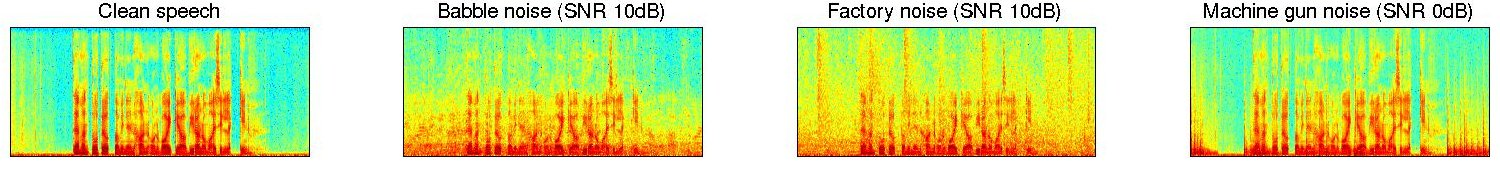
\includegraphics[width=\textwidth]{images/natural_spectra.jpg}
\caption{Natural speech FFT spectra of clean speech, speech with babble noise, factory noise and machine gun noise}
\label{fig:natural_spectra}
\end{centering}
\end{figure}

Figure \ref{fig:natural_spectra} shows the spectra of a natural speech sample in different environmental conditions while Figure \ref{fig:synthetic_spectra} shows the spectra of the same samples resynthesized with GlottHMM.

\begin{figure}[!htb]
\begin{centering}
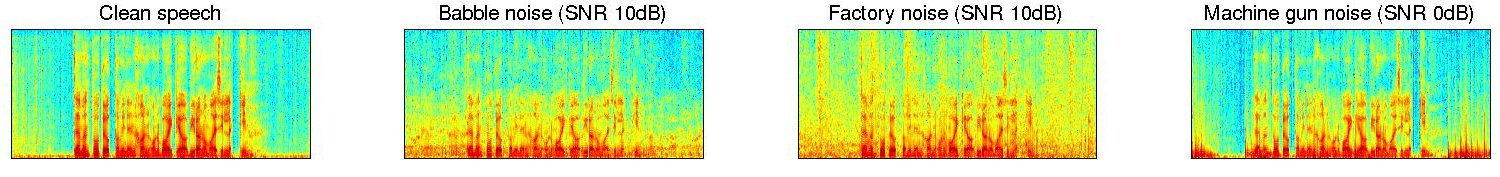
\includegraphics[width=\textwidth]{images/synthetic_spectra.jpg}
\caption{Synthetic speech FFT spectra of clean speech, speech with babble noise, factory noise and machine gun noise after analysis and resynthesis with GlottHMM}
\label{fig:synthetic_spectra}
\end{centering}
\end{figure}

As it can be seen, both the natural and the synthetic spectra has little differences between them.
%
%
After listening to the samples we could conclude that noise was not influencing the regular performance GlottHMM.

Another important issue is finding a correct configuration for GlottHMM.
%
In Appendix \ref{glott_conf_file}, the configuration file needed by GlottHMM can be found.
%
This file has a great amount of options to configure. 
%
However, thanks to previous experiments conducted and the advice of Tuomo Raitio, who developed GlottHMM, the tweaks to make in the configuration file are focused in noise robustness and some voice characteristics.

Some low $F_{0}$ problems were noticed during the first rounds of experiments.
% 
This problems consisted of frames where the voice sounded funny.
%
To find out the details of this issue, a simple $F_{0}$ histogram plotting was made.
%
Figure \ref{fig:f0_histograms} presents the histograms of the voices used to build the average voice model, where low-frequency peaks can be pointed out in some of the voices.

\begin{figure}[!htb]
\begin{centering}
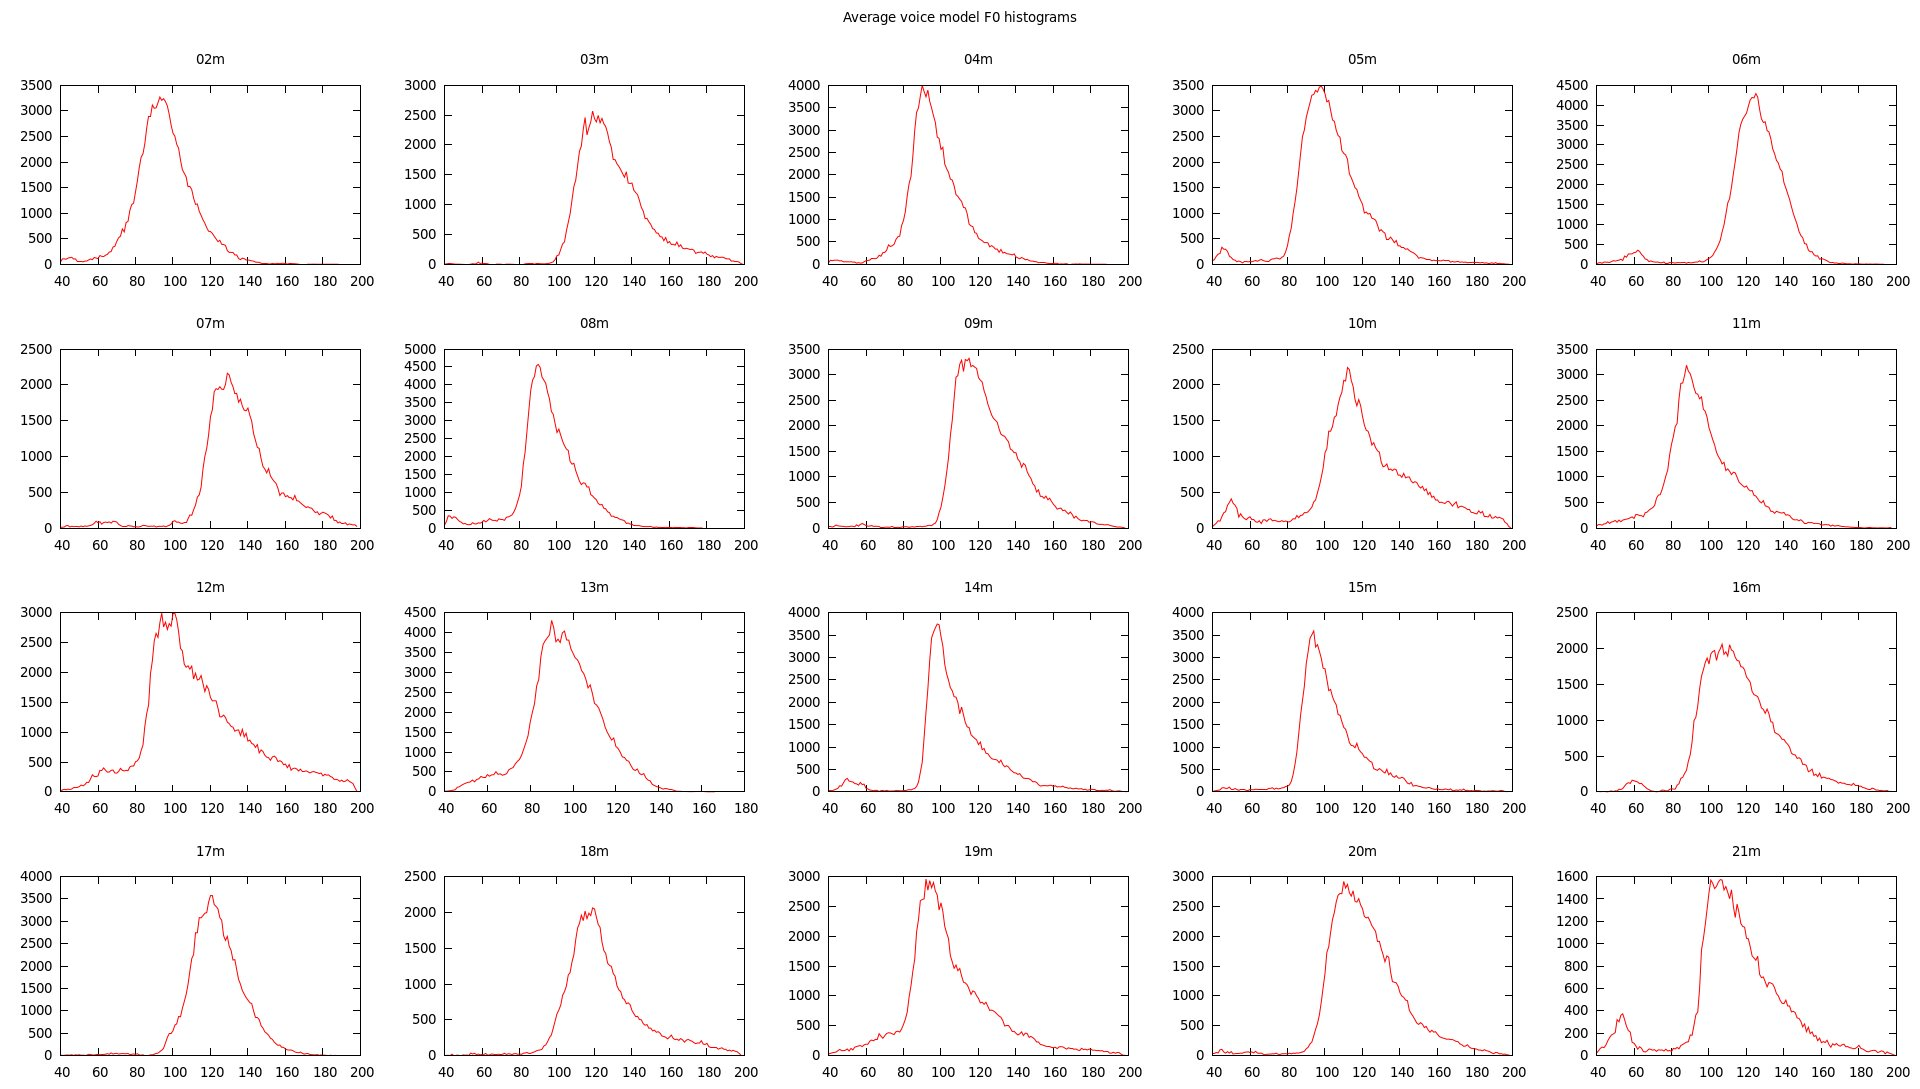
\includegraphics[width=\textwidth]{images/av_model_=conf_f0_histogram.jpg}
\caption{$F_{0}$ histogram of the voices composing the average voice model}
\label{fig:f0_histograms}
\end{centering}
\end{figure}

Solving this problem only required to extract again the features for the voices with low-frequency peaks.
%
These peaks were found around 40-60 Hz in the training data, used in the average voice model, and in the adaptation data.
%
To eliminate them, in the configuration file the $F_{0}$ lower-limit was set to 65 Hz.

The last round of initial experiments conducted aim to find the best combination of the noise reduction parameters shown in Appendix \ref{glott_conf_noise_red}.
%
These experiments consist on analysis and resynthesis of the noisy data varying the parameters in Appendix \ref{glott_conf_noise_red} and carrying out the objective measures described in \ref{evaluation_objective}.
%

\begin{figure}[!htb]
\begin{centering}
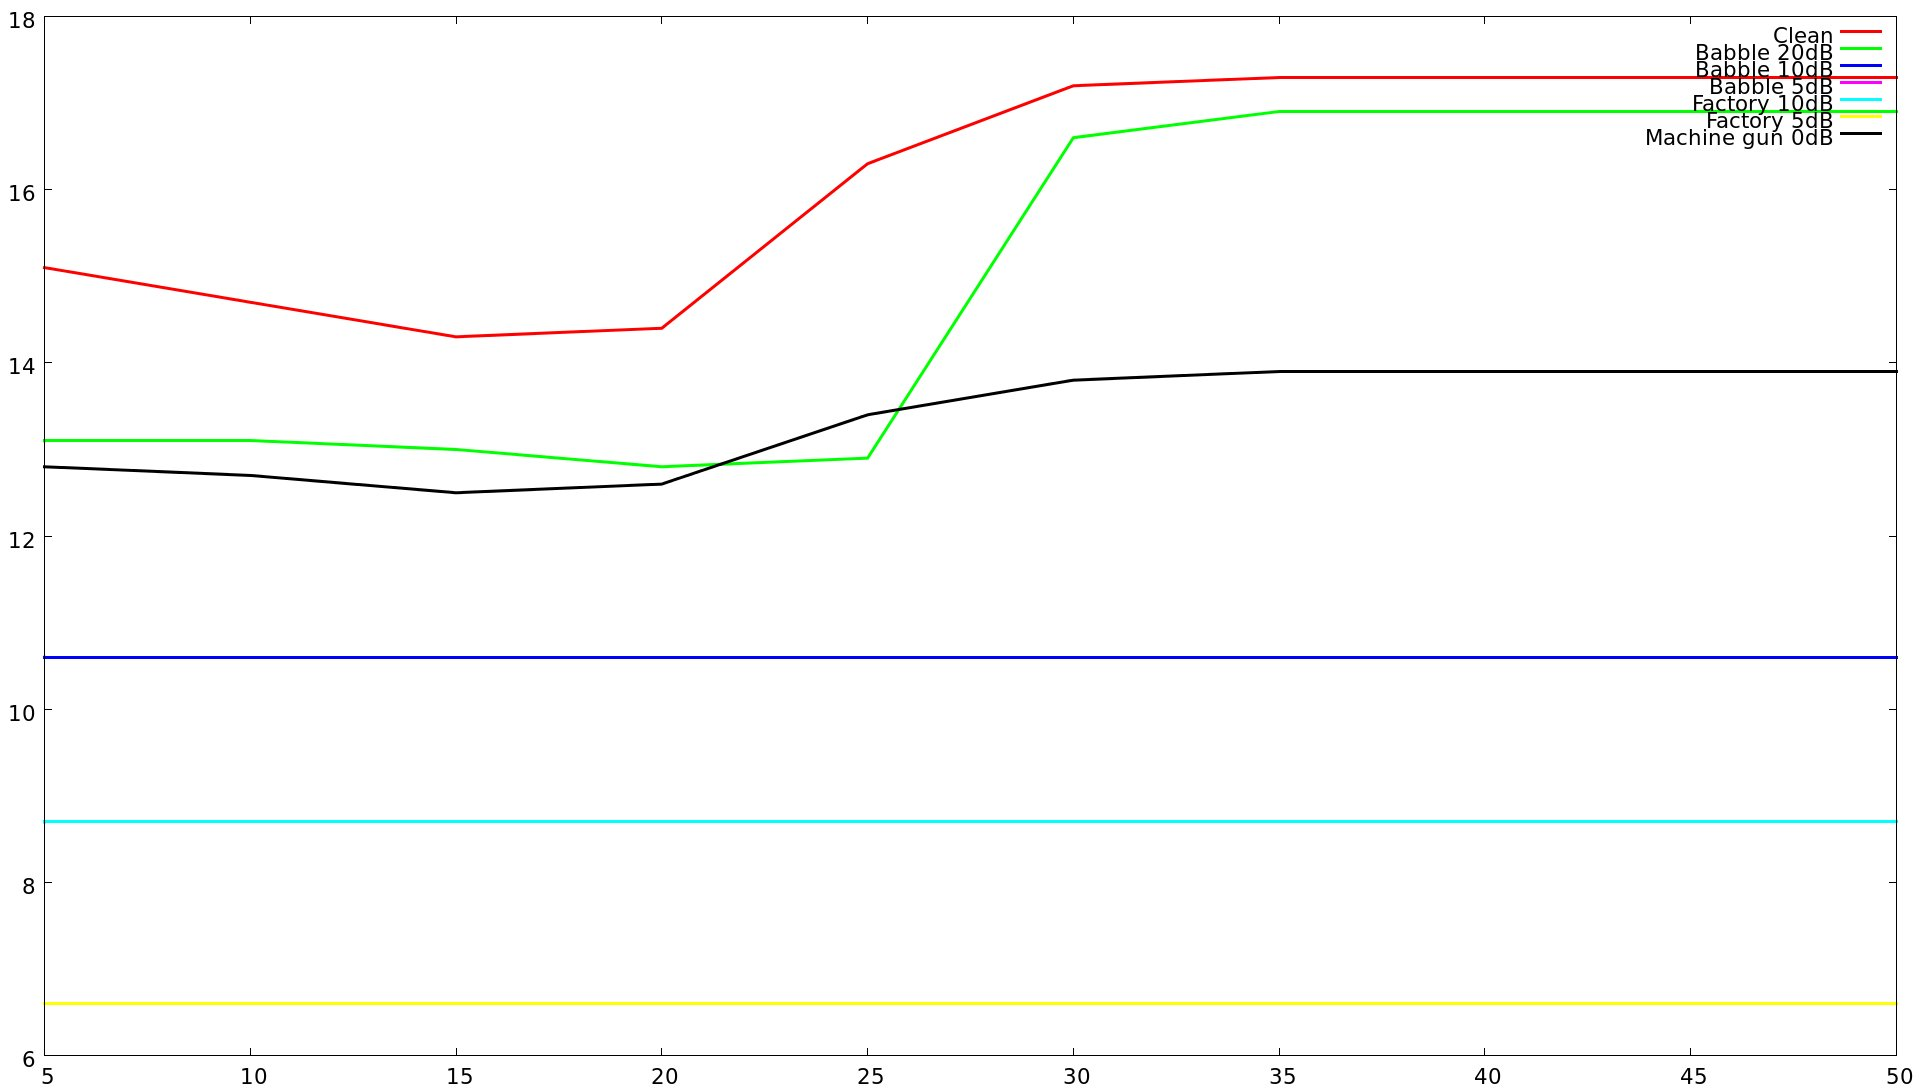
\includegraphics[width=\textwidth]{images/noise_red_snr_exp.jpg}
\caption{SNR measures with $NOISE\_REDUCTION\_LIMIT = 4.5$ fixed and $NOISE\_REDUCTION\_DB$ from 5 to 50}
\label{fig:noise_red_snr}
\end{centering}
\end{figure}

\begin{figure}[!htb]
\begin{centering}
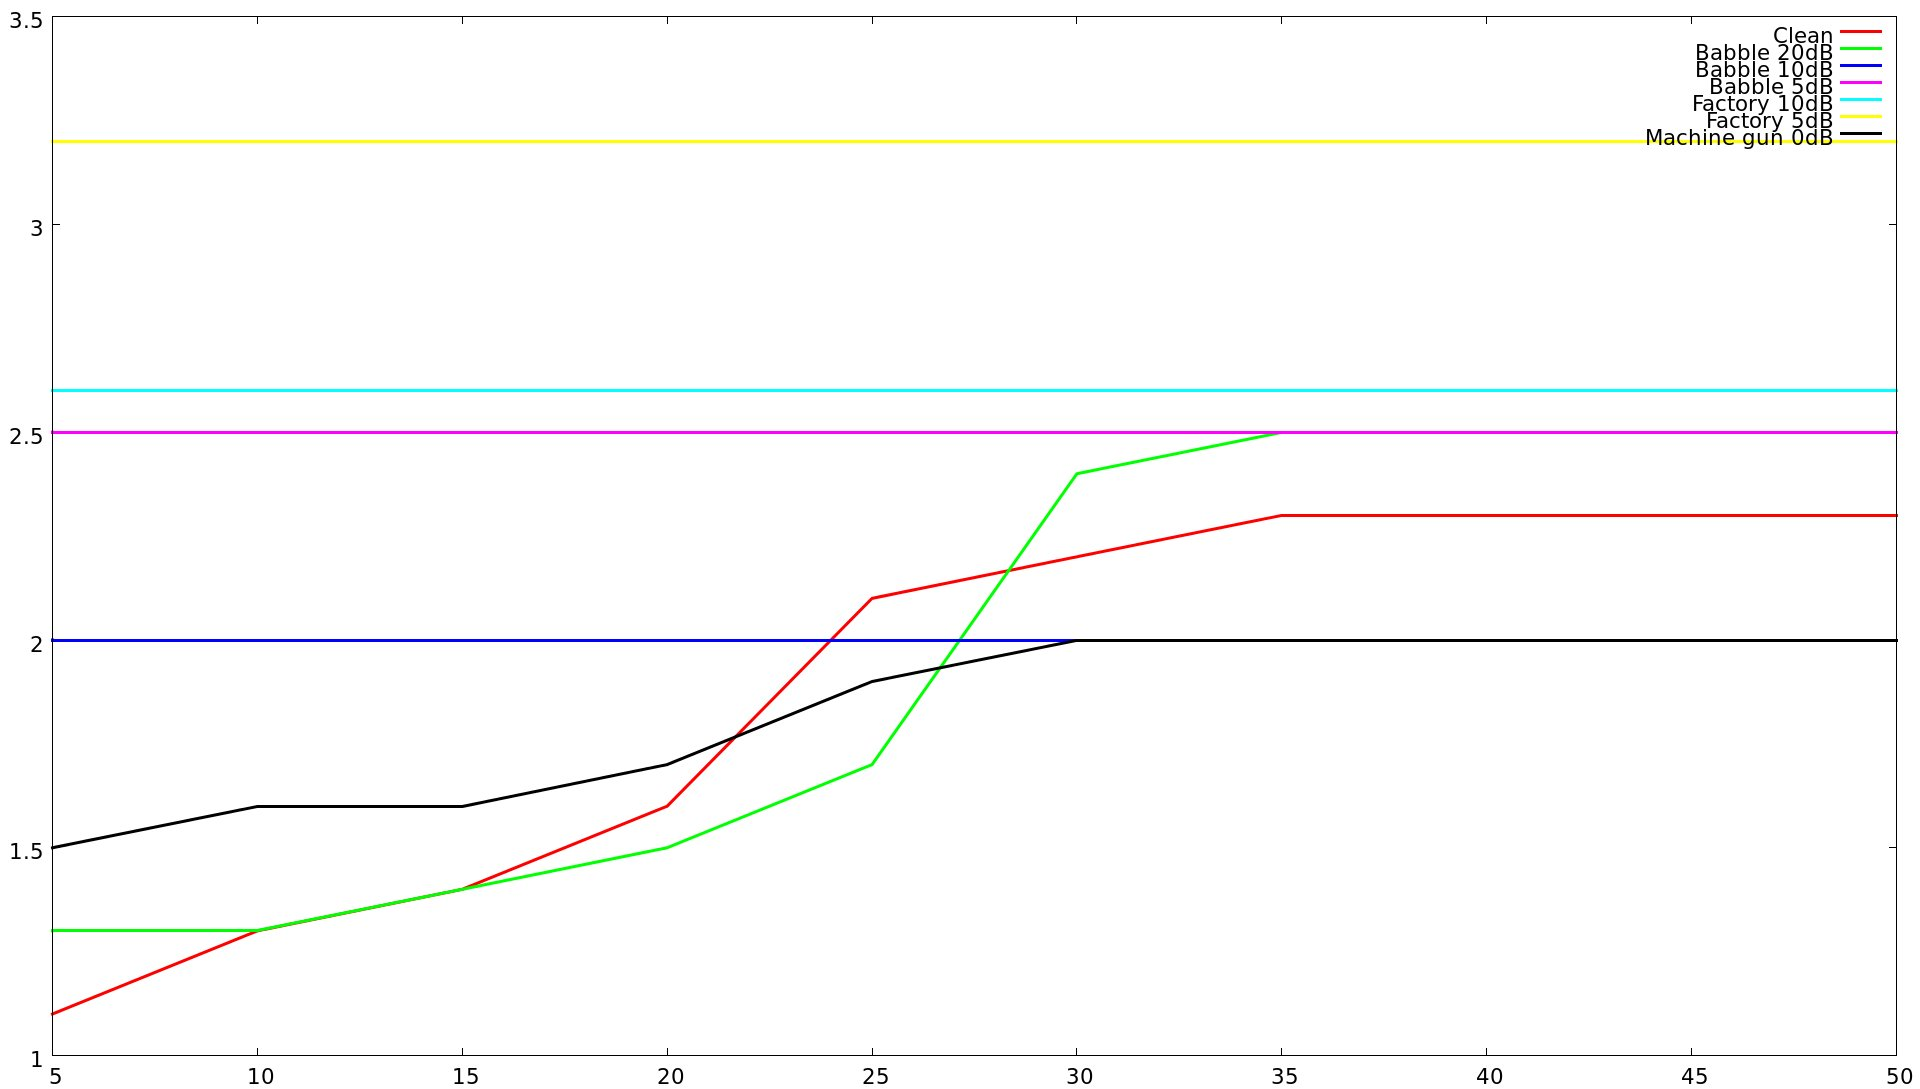
\includegraphics[width=\textwidth]{images/noise_red_mcd_exp.jpg}
\caption{MCD measures with $NOISE\_REDUCTION\_LIMIT = 4.5$ fixed and $NOISE\_REDUCTION\_DB$ from 5 to 50}
\label{fig:noise_red_mcd}
\end{centering}
\end{figure}

\begin{figure}[!htb]
\begin{centering}
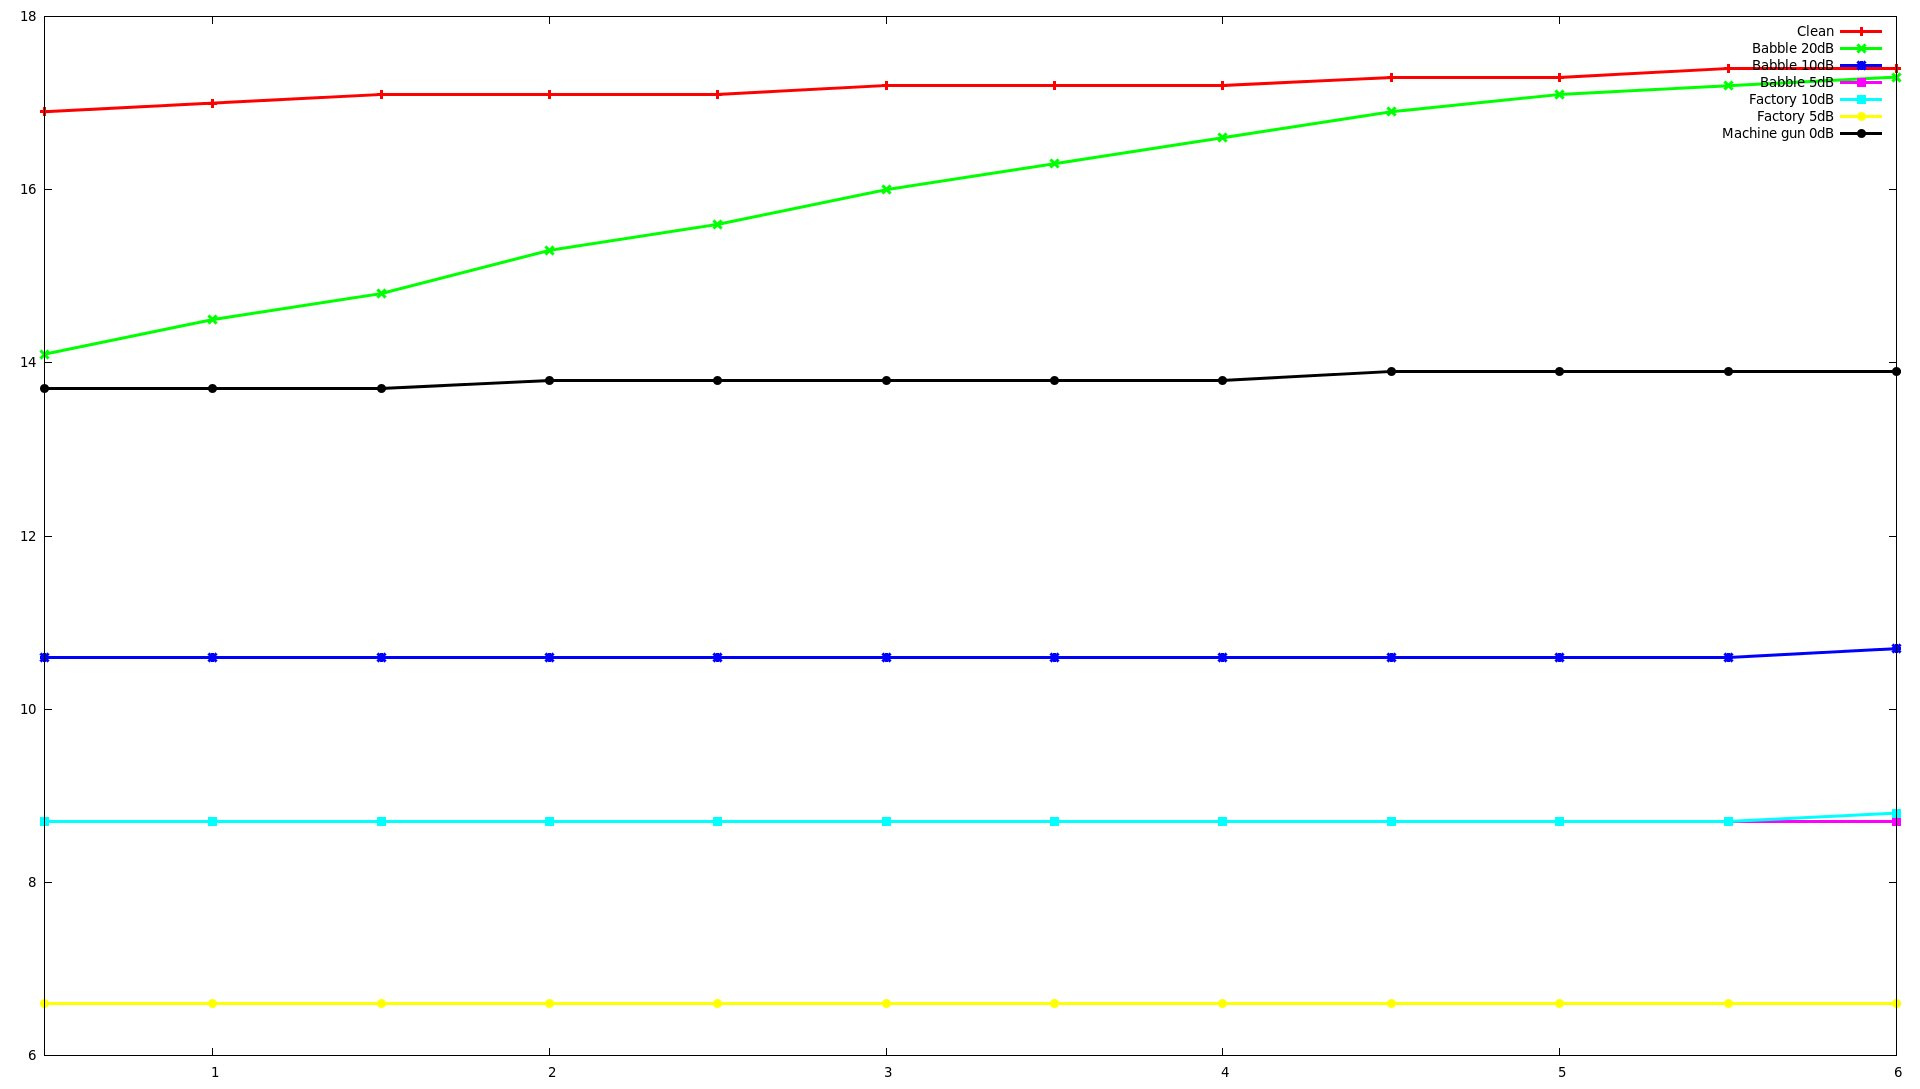
\includegraphics[width=\textwidth]{images/noise_red_lim_snr_exp.jpg}
\caption{SNR measures with $NOISE\_REDUCTION\_DB = 35$ fixed and $NOISE\_REDUCTION\_LIMIT$ from 0.5 to 6}
\label{fig:noise_red_lim_snr}
\end{centering}
\end{figure}

\begin{figure}[!htb]
\begin{centering}
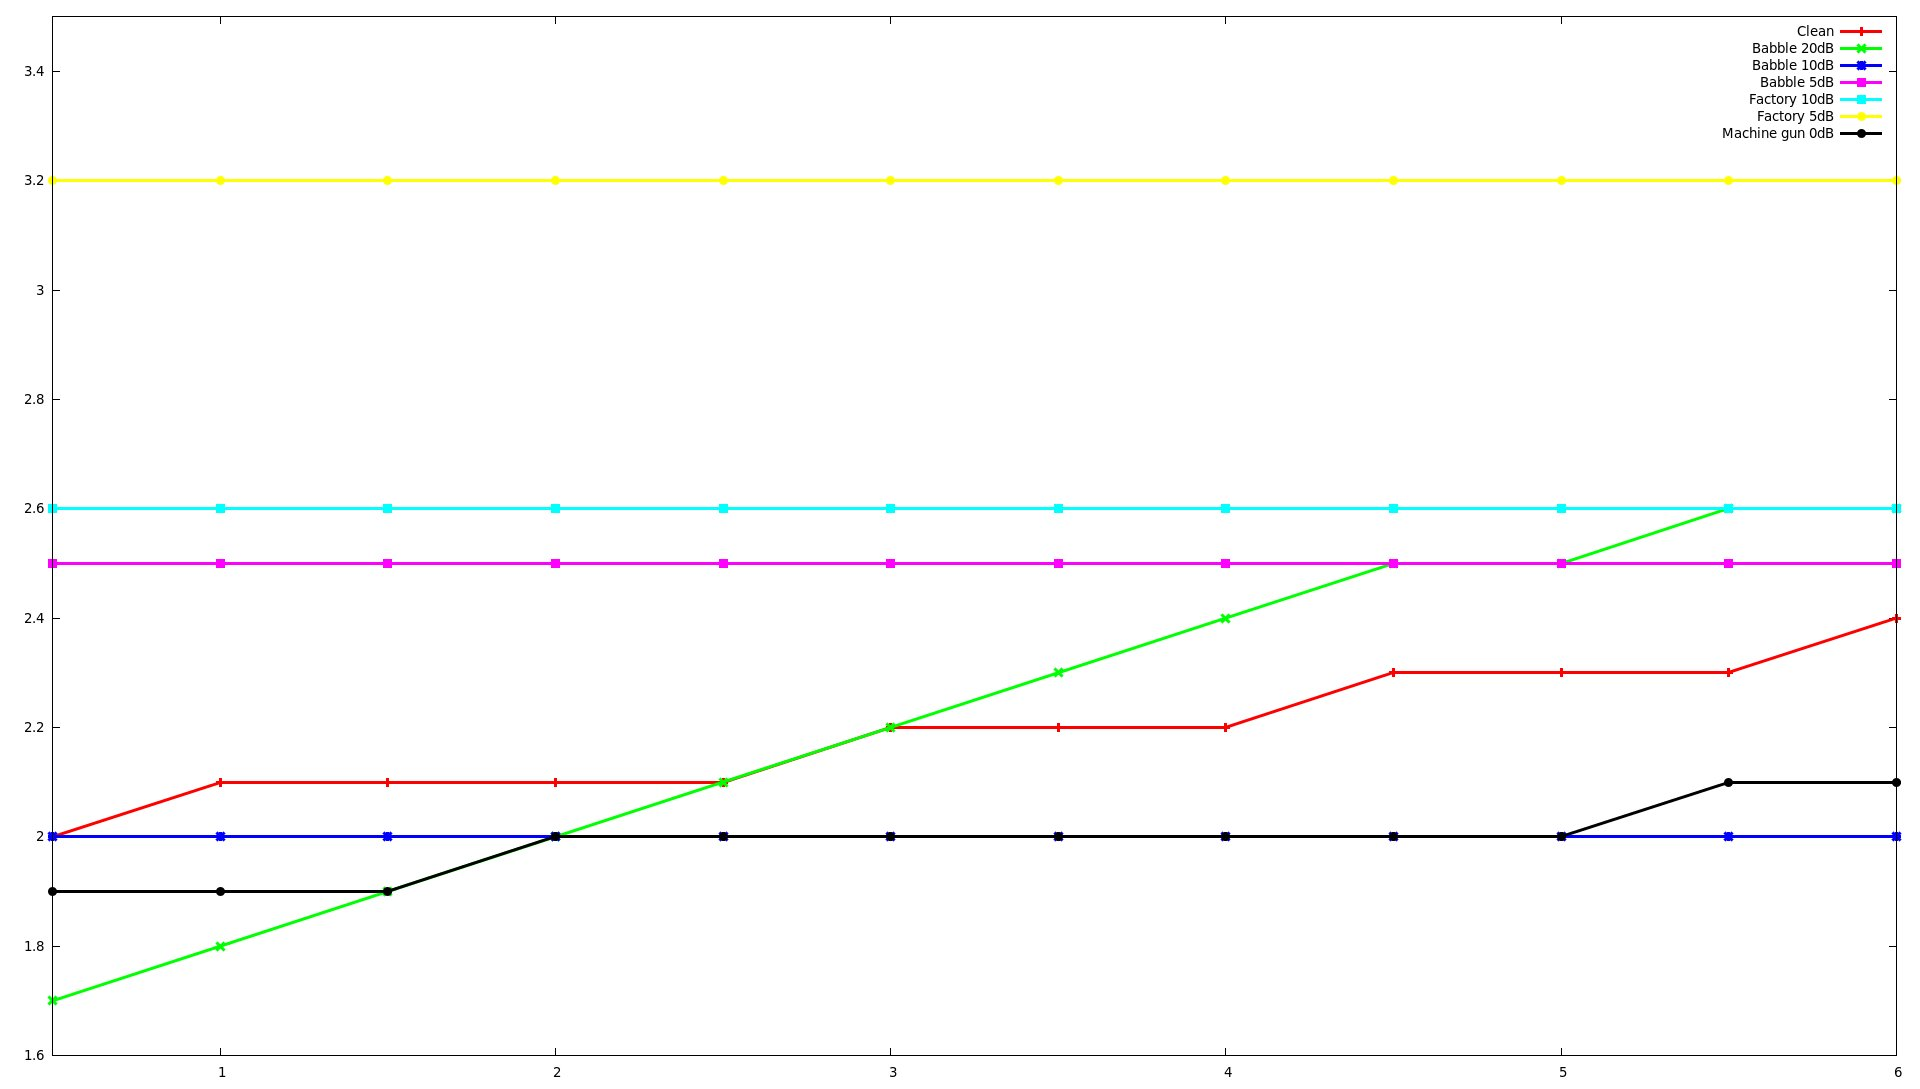
\includegraphics[width=\textwidth]{images/noise_red_lim_mcd_exp.jpg}
\caption{MCD measures with $NOISE\_REDUCTION\_DB = 35$ fixed and $NOISE\_REDUCTION\_LIMIT$ from 0.5 to 6}
\label{fig:noise_red_lim_mcd}
\end{centering}
\end{figure}
Figures \ref{fig:noise_red_snr}, \ref{fig:noise_red_mcd}, \ref{fig:noise_red_lim_snr} and \ref{fig:noise_red_lim_mcd} illustrate the evolution of the SNR and MCD measures when varying NOISE\_REDUCTION\_DB with a fixed NOISE\_REDUCTION\_LIMIT and vice versa.
%
As it can be seen in Figure \ref{fig:noise_red_snr}, for a fixed noise reduction limit the SNR measures increase significantly (higher SNR scores mean better quality) between 20 and 35dB noise reduction for the cases of clean and babble 20dB samples, reaching a limit.
%
Also, there is a slight improvement in the case of machine gun 0dB noise, but in the rest of the cases no improvement is seen.
%
As SNR scores increase MCD follows a similar patter (higher MCD scores mean worse quality).
%
In Figure \ref{fig:noise_red_mcd} it can be seen that the cases where the SNR was increasing are the ones with an increase of the MCD scores.
%
The ones with steady SNR scores have no changes in the MCD either.

The case where NOISE\_REDUCTION\_DB is fixed and the variation is made in the NOISE\_REDUCTION\_LIMIT is presented in Figures \ref{fig:noise_red_lim_snr} and \ref{fig:noise_red_lim_mcd}.
%
When increasing the NOISE\_REDUCTION\_LIMIT a steady increase of the SNR scores is only appreciable in the case of babble 20dB background samples.
%
All the other cases remain stable, although a very small increase, not significant, can be spot for clean and machine gun 0dB cases.
%
MCD scores follow the same pattern explained before. 
%
Babble 20dB has both increases in SNR and MCD.
% 
Not so big as in babble 20dB case increases in MCD can be found also for the clean and machine gun cases, probably due to the small improvement appreciated in their SNR.

A frame by frame representation of the natural waveform, resynthesized waveforms and SNR and MCD measures for the cases of babble 10dB and 20 dB background noise is shown in Figures \ref{fig:frame_by_frame_babble10} and \ref{fig:frame_by_frame_babble20}.

\begin{figure}[!htb]
\begin{adjustwidth}{-2.6cm}{}
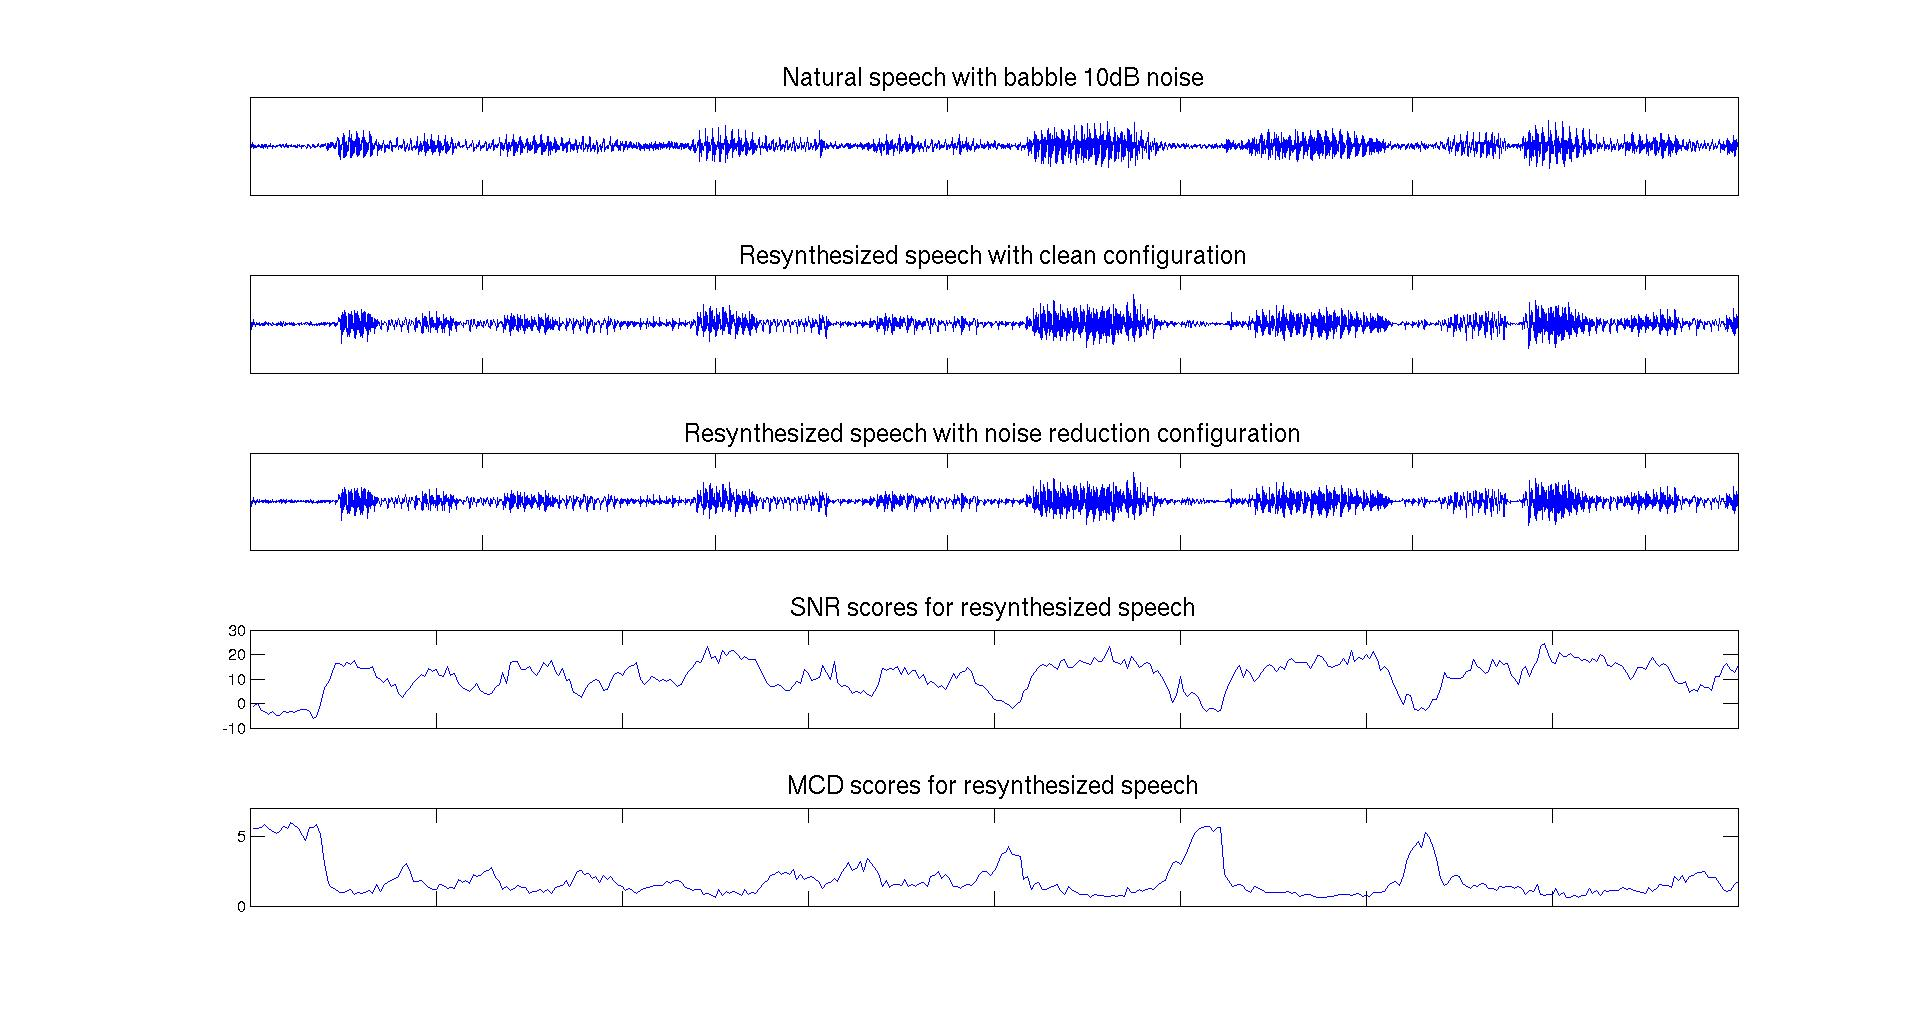
\includegraphics[width=1.3\textwidth]{images/babble10_frame_by_frame.jpg}
\end{adjustwidth}
\caption{Frame by frame representation of the natural speech with a babble background noise level of 10dB, resynthesized speech after analysis with GlottHMM not using the noise reduction module, resynthesized speech using the noise reduction module and SNR and MCD measures for both synthetic samples}
\label{fig:frame_by_frame_babble10}
\end{figure}

\begin{figure}[!htb]
\begin{adjustwidth}{-2.6cm}{}
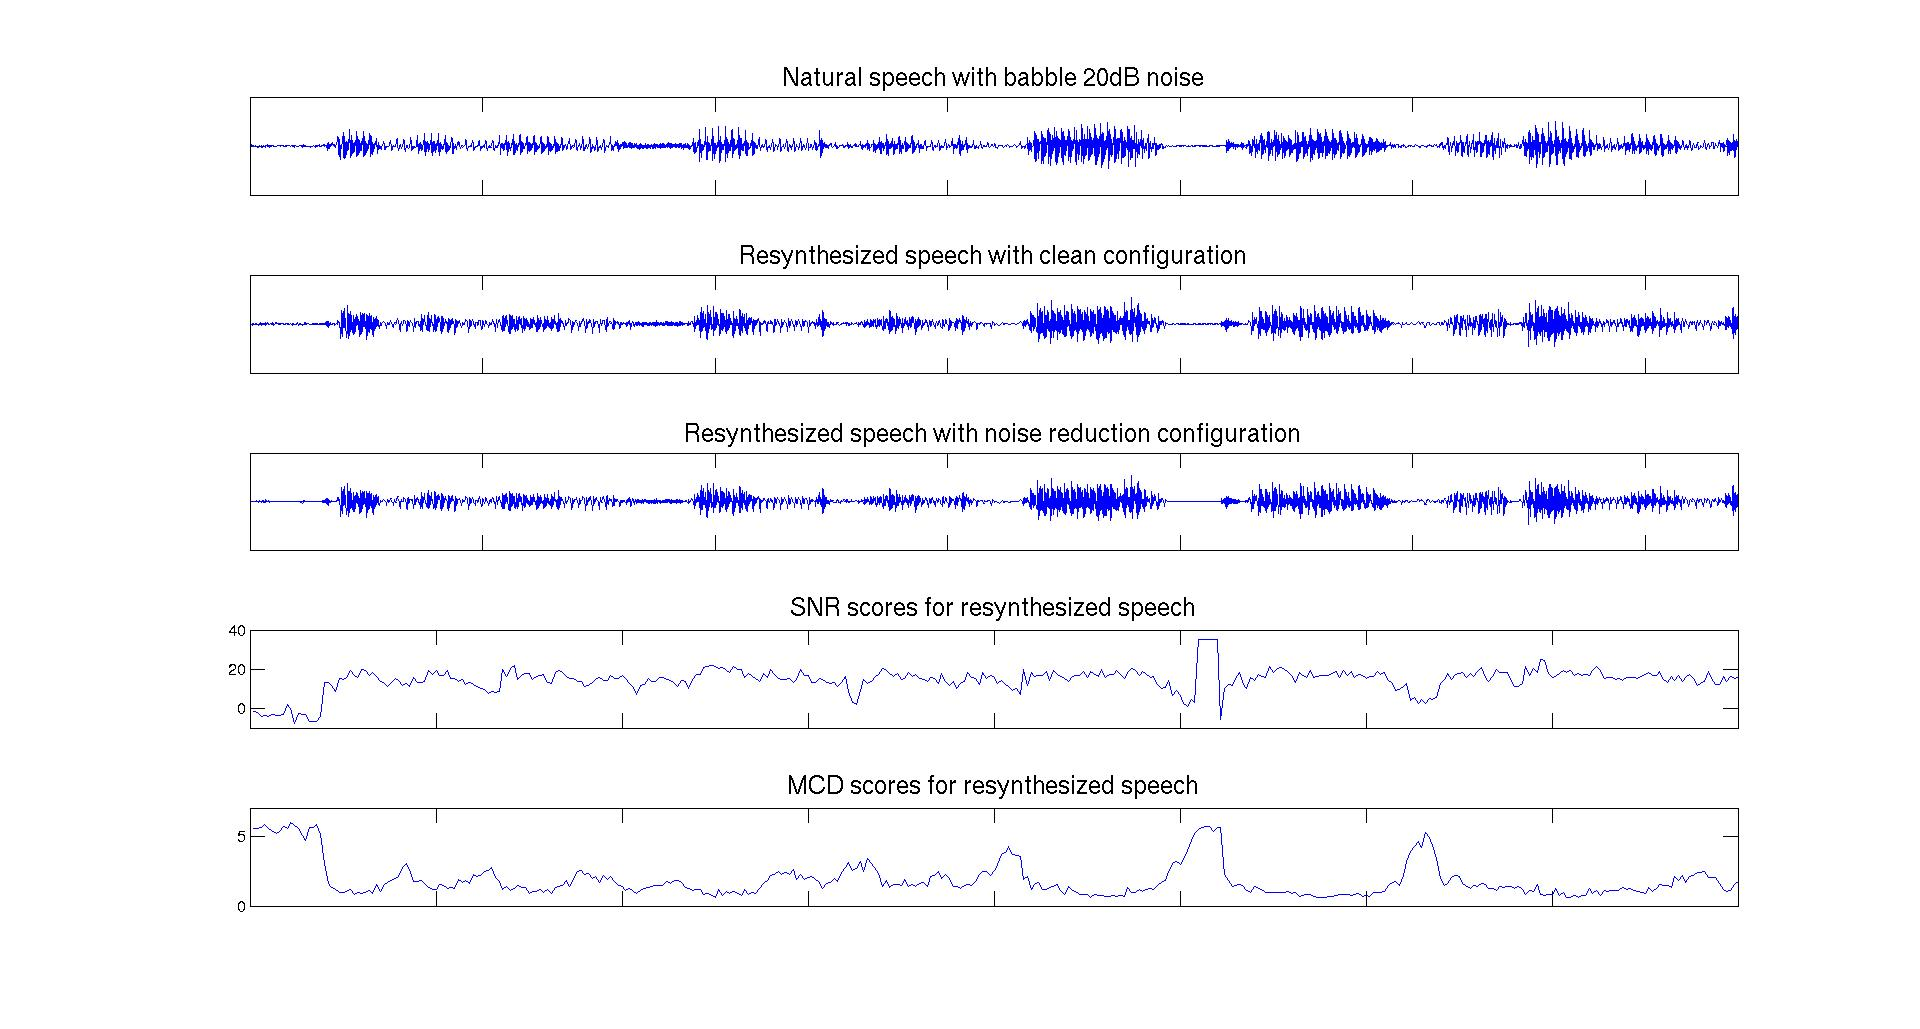
\includegraphics[width=1.3\textwidth]{images/babble20_frame_by_frame.jpg}
\end{adjustwidth}
\caption{Frame by frame representation of the natural speech with a babble background noise level of 20dB, resynthesized speech after analysis with GlottHMM not using the noise reduction module, resynthesized speech using the noise reduction module and SNR and MCD measures for both synthetic samples}
\label{fig:frame_by_frame_babble20}
\end{figure}

In the case of the waveforms, we can see no difference when the data is corrupted with a 10dB level babble noise, while when the background noise level is 20dB the noise reduction module used by GlottHMM results in an improvement of the quality attending to cleaner synthetic waveform in speech silences and better objective measures, visible for example when the SNR reaches its maximum value (35 dB). 

A comparison between the measures done when resynthesizing using the noise reduction module and without using it is shown in Figures \ref{fig:babble10_clean_vs_noise} and \ref{fig:babble20_clean_vs_noise}. 
%
No significant difference can be spotted when talking about the babble 10dB case.
%
Nevertheless, in the case of having a babble 20dB background noise, we can point out different frames where the noise reduction module is clearly improving the SNR quality (careful with the different scales in the graph).
%
Some frames reach the maximum SNR value (35 dB) while when not using the noise reduction module the same frames form a valley in the SNR graph.
%
Other examples of this behavior can be found at the graph.

However, the MCD measures in those cases are contradictory. 
%
While the SNR increases, meaning a quality improvement, the MCD also increases creating the opposite effect, a quality decrease.

From all these initial experiments it can be said that the noise reduction included in the GlottHMM vocoder is not capable of carrying out its function when severe noise conditions are found.
%
However, when the noise conditions are reasonable to record audio, these first experiments show that GlottHMM gets along quite well in analysis and resynthesys, potentially improving the quality when adapting an HMM-based system. 

\begin{figure}[!htb]
\begin{adjustwidth}{-2.6cm}{}
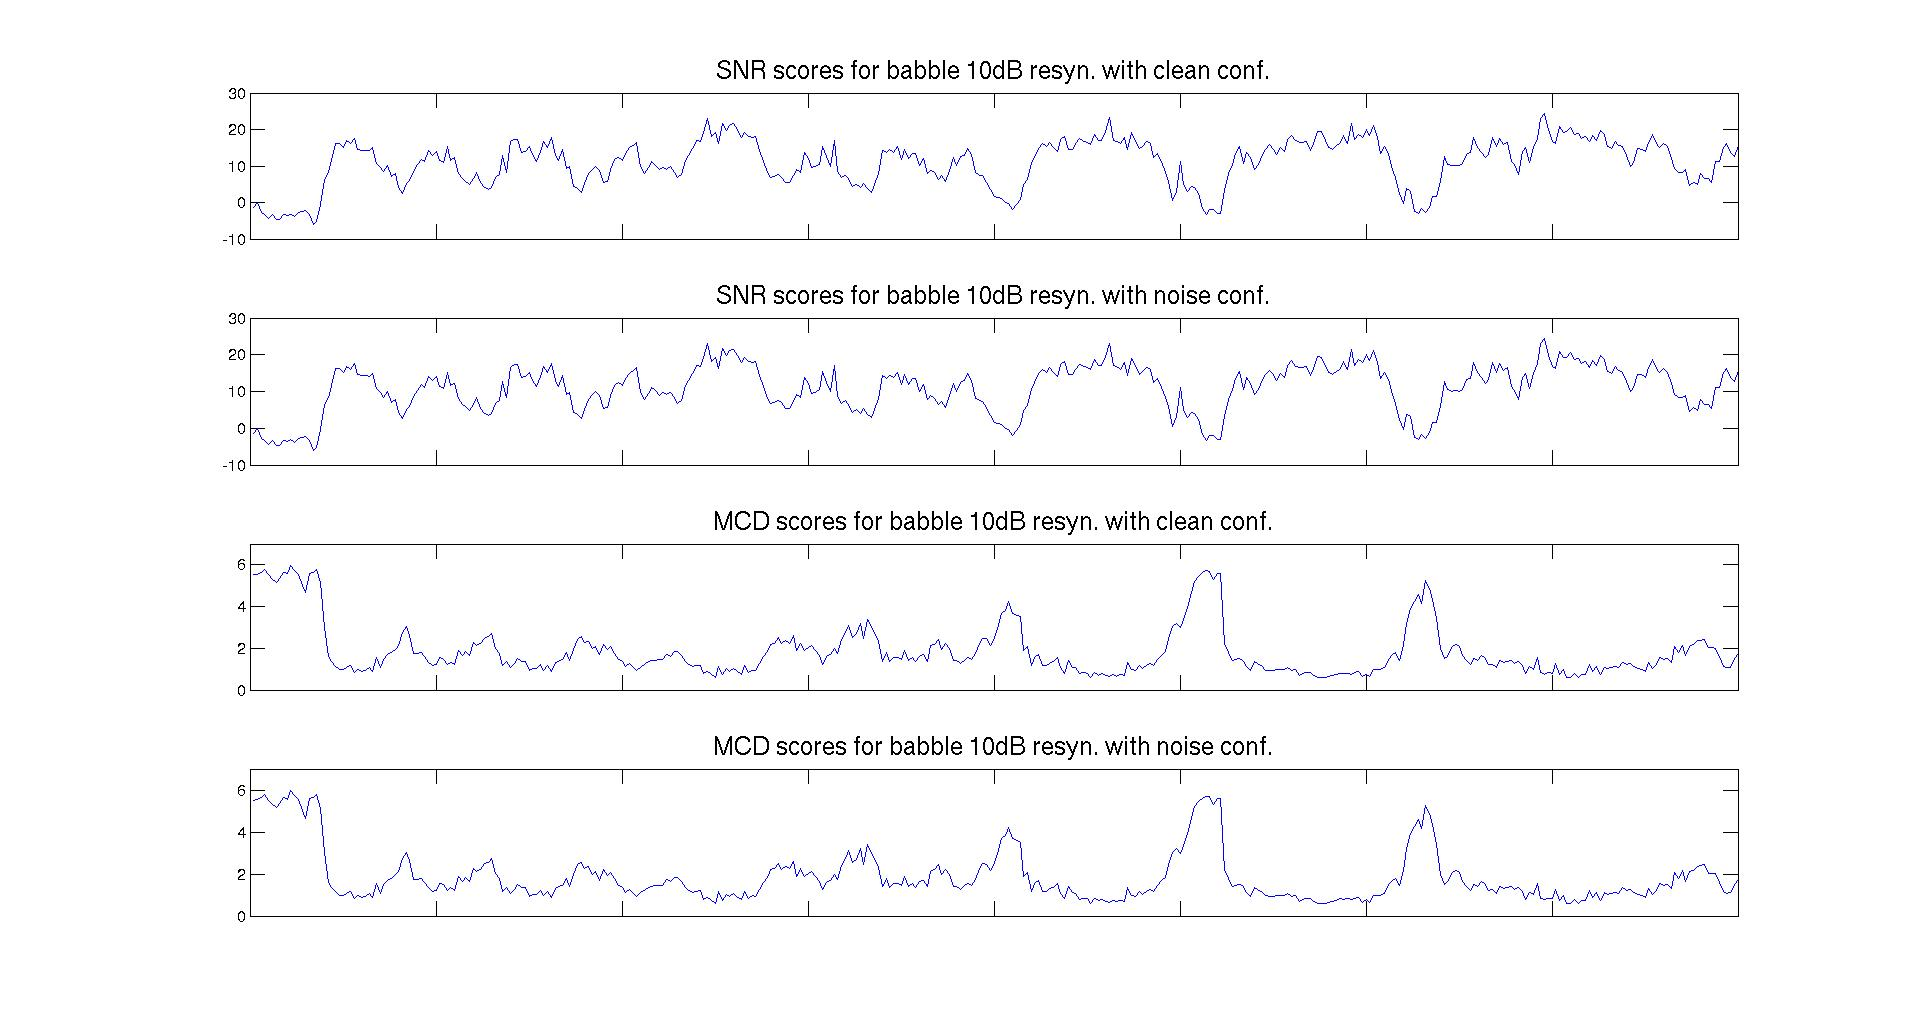
\includegraphics[width=1.3\textwidth]{images/babble10clean_vs_noise.jpg}
\end{adjustwidth}
\caption{SNR and MCD measures of a resynthesized sample with babble 10dB background noise using and not using the noise reduction module}
\label{fig:babble10_clean_vs_noise}
\end{figure}

\begin{figure}[!htb]
\begin{adjustwidth}{-2.6cm}{}
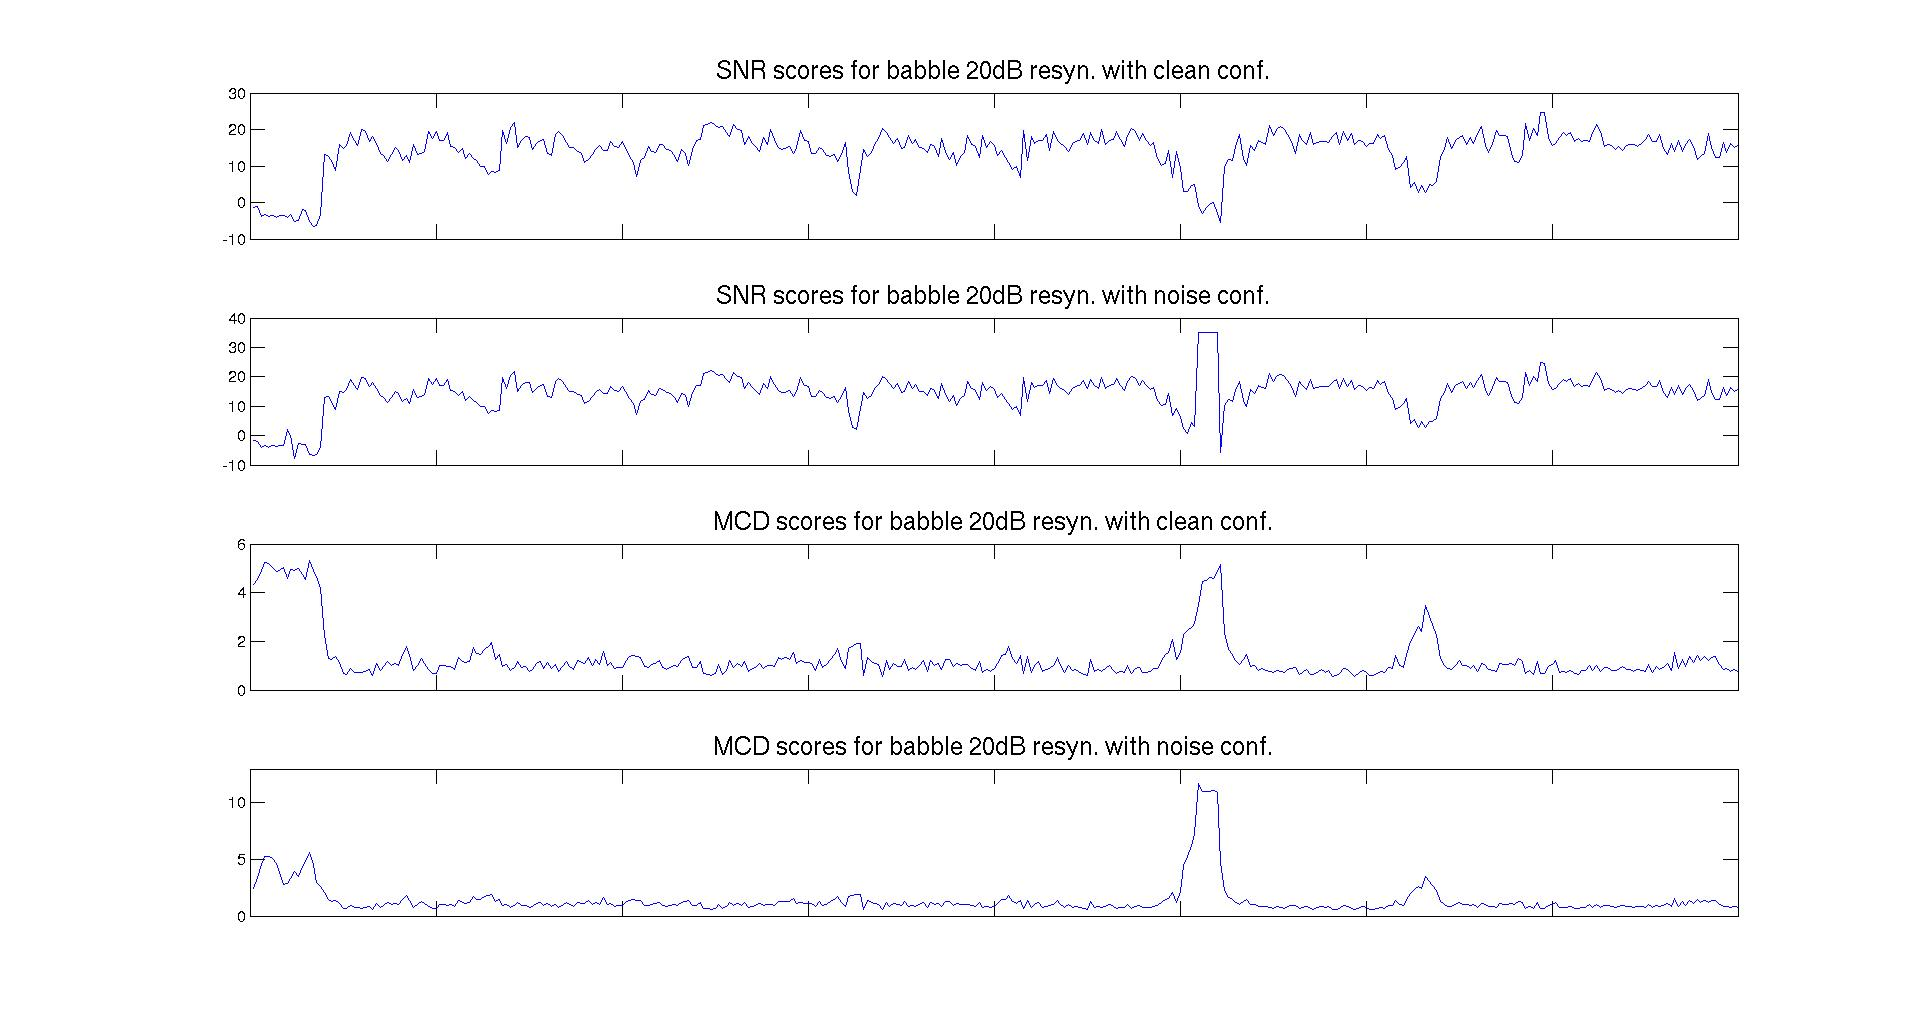
\includegraphics[width=1.3\textwidth]{images/babble20clean_vs_noise.jpg}
\end{adjustwidth}
\caption{SNR and MCD measures of a resynthesized sample with babble 20dB background noise using and not using the noise reduction module}
\label{fig:babble20_clean_vs_noise}
\end{figure}

\subsection{Average Voice Model}
\label{experiments_av_voice_model}
